\chapter{Optization of Association Hyperparameters}

\section{Definition of the Association Error}

% Like in Chap 4, a small introduction of the association error, including first and second type of the error and the harmonic averange of the error. 

A correct association constructs one-to-one correspondence between the tracks and the particles. When the correspondence is violated, there are association errors.

The association error contains error of the first and second kind. We define the first kind of error $E_{1}$ as a track including the measurements which should belong to other tracks. An example
is depicted in Figure \ref{asso err}b. An error is called the second kind of error $E_{2}$ when is that a measurement is assigned to a wrong track, as illustrated in Figure \ref{asso err}c \cite{pfaff2019multitarget}. The harmonic mean of both errors $E_{mean}=\frac{2E_{1}E_{2}}{E_{1}+E_{2}}$ is used in  the following part for explaining the general accuracy of the association. 


\begin{figure}[htbp]
\centering
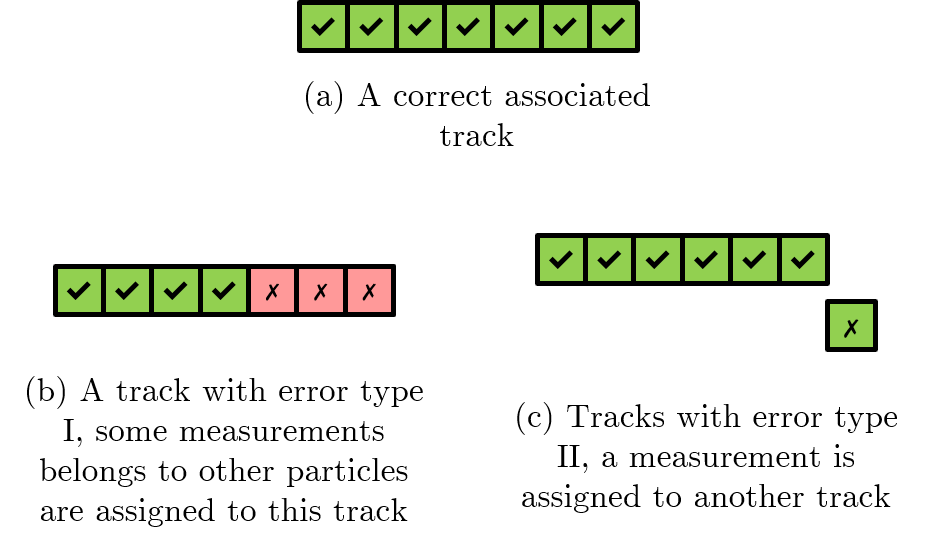
\includegraphics[width=0.7\textwidth]{figures/Asso/association error.png}
\caption{Illustrations for the two types of association errors. The  color of the cells indicates the ID of the actual particle from which the measurement stems, adapted from \cite{pfaff2019multitarget}}
\label{asso err}
\end{figure}

Tracking errors can be caused by different factors. For example, when two particle collide, the measurements from both particles can exchange to the tracks from another particle, as illustrated in Figure \ref{asso err2}a. Another example is that a particle is assigned to two separated tracks. It can occurred when the particle is not observed in some frames, as depicted in Figure \ref{asso err2}b. But even if the measurements are continuous, this type of error can still happen when the prediction is too far away from the measurement or the association hyperparameters are chosen beyond the reasonable range, as shown in Figure \ref{asso err2}c. 

\begin{figure}[htbp]
\centering
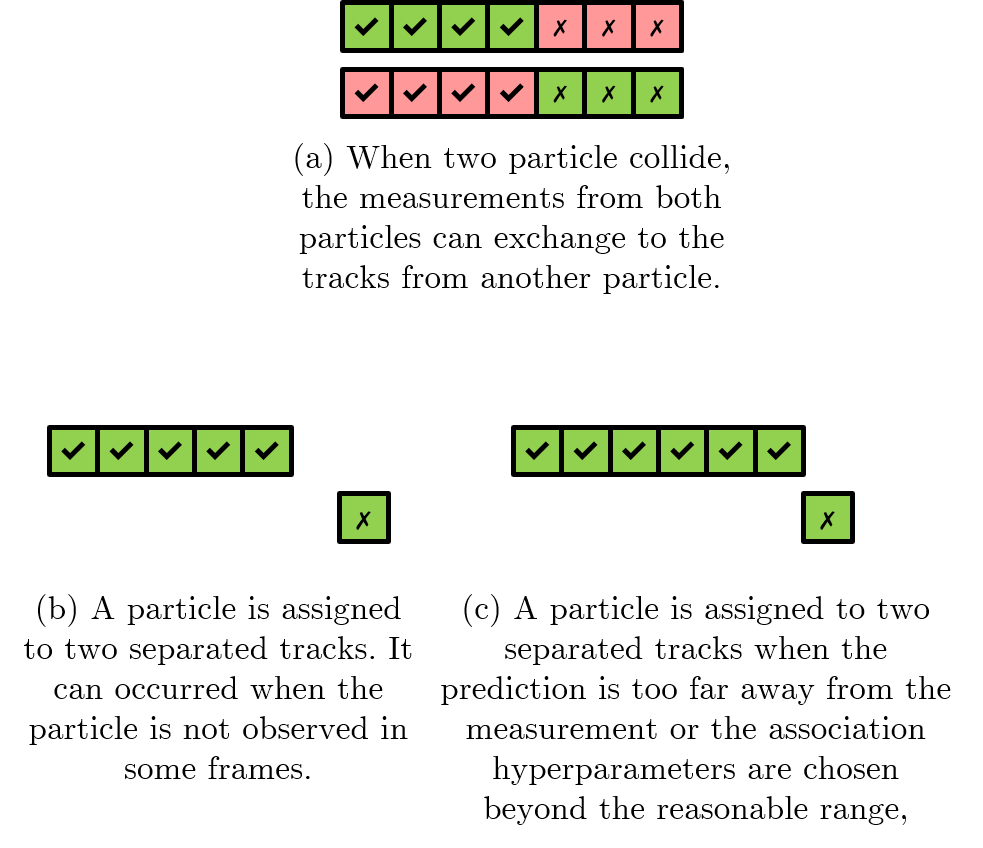
\includegraphics[width=0.7\textwidth]{figures/Asso/association error2.png}
\caption{Illustrations of some typical association errors, adapted from \cite{pfaff2019multitarget}}
\label{asso err2}
\end{figure}


\section{Effect of the Hyperparameters}

Like in Chap 4, each hyperparameter is tested with the grid-search-like method, in order to find the effect of each hyperparameter.

One small paragraph for explaining the "robust range". The aim of this chapter is not to find best hyperparameters, but an acceptable range of these HPs.


\section{Robust Range of Association Hyperparameters}

(Results with SVM)

First describe the method (collecting training data, setting of function and something else).

Several plots like this. After plots give some analyse (). 

\begin{figure}[htbp]
\centering
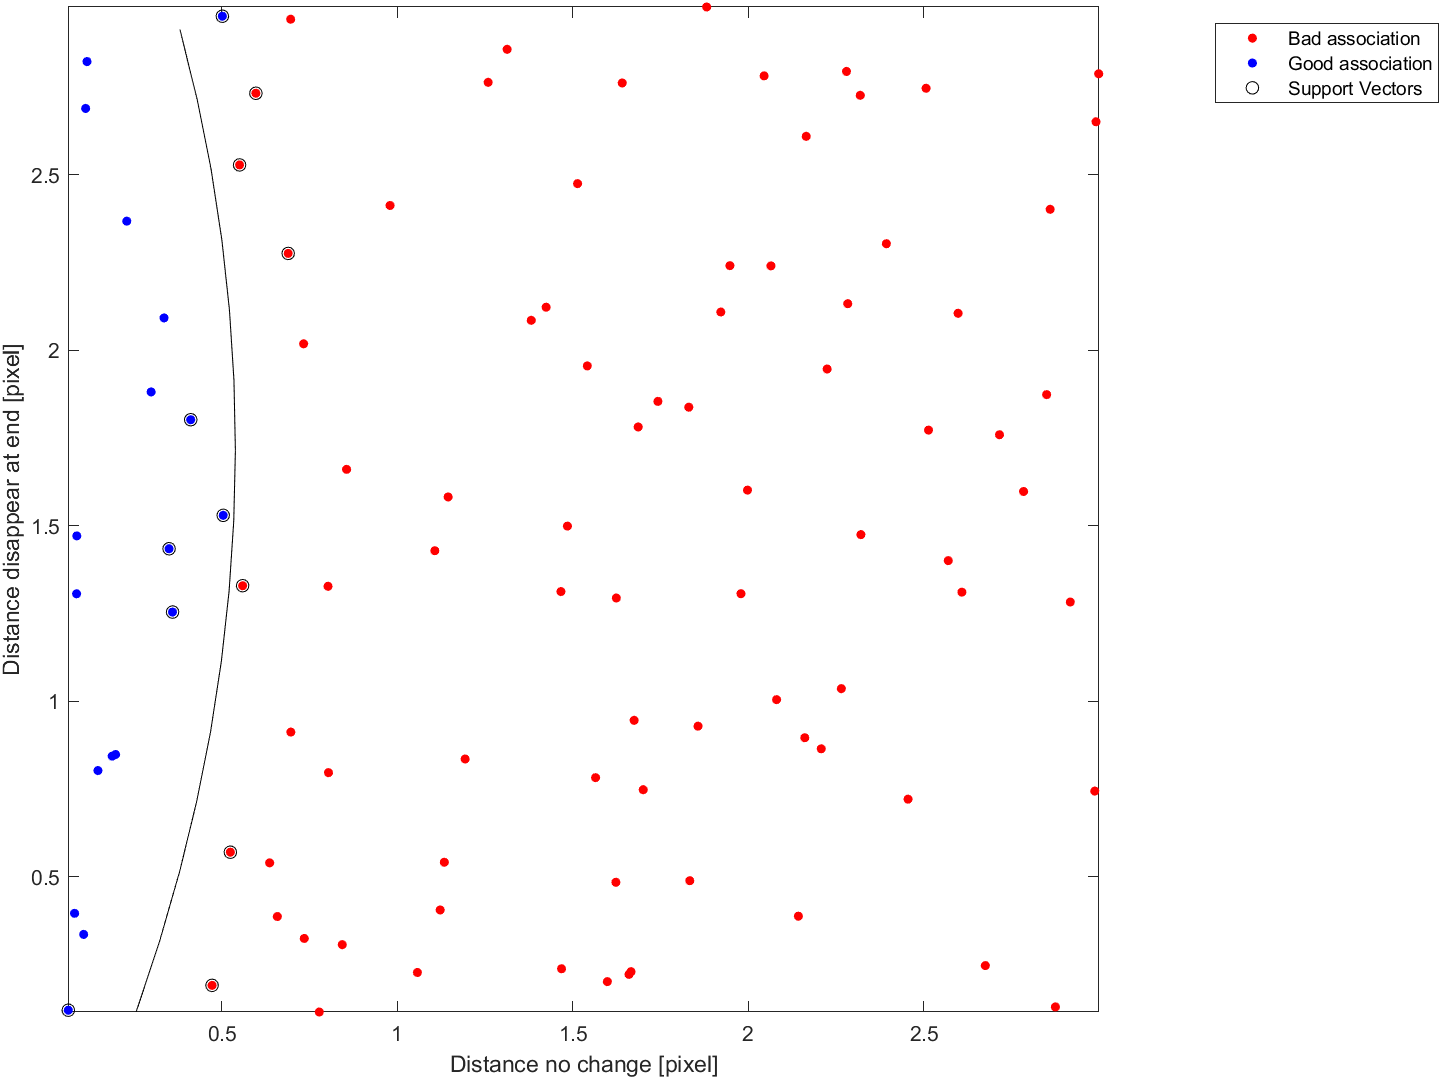
\includegraphics[width=0.9\textwidth]{figures/Asso/sample SVM.png}
\caption{need to change into the version with the colors showing the error rate}
\label{svm1}
\end{figure}